\documentclass[a4paper, 12pt]{article}
\usepackage[utf8]{inputenc}
\usepackage{amsmath}
\usepackage{graphicx}
\usepackage{float}  % Pakiet umożliwiający kontrolę położenia obrazów
\usepackage{caption} % Umożliwia dostosowanie podpisów pod obrazami
\usepackage{hyperref}
\usepackage{geometry}
\usepackage[T1]{fontenc} % Żeby działały polskie "ogonki"
\usepackage[labelformat=simple]{caption}
\geometry{margin=1in}


% Tytuł i autor
\title{Raport z ćwiczenia NUM1\\numeryczne przybliżenie pochodnej funkcji}
\author{Bartosz Satoła}
\date{15.10.2024}

\begin{document}

\maketitle
\tableofcontents
\newpage

\section{Cel ćwiczenia}
Celem ćwiczenia było zbadanie błędu przybliżenia numerycznego pochodnej funkcji \( f(x) = \sin(x^3) \), stosując dwie różne metody.
Wyniki zostały porównane z dokładną wartością pochodnej (wyliczonej z odpowiednich wzorów używanych w analizie matematycznej) w celu oceny dokładności obu metod w zależności od kroku \( h \).

\section{Opis ćwiczenia}
W ramach ćwiczenia zaimplementowano funkcje obliczające numerycznie pochodne funkcji \( f(x) = \sin(x^3) \) dla zmiennych typu \texttt{float} oraz \texttt{double}, z wykorzystaniem dwóch metod:
\begin{itemize}
    \item Metody różnic w przód,
    \item Metody różnic centralnych.
\end{itemize}

Dla obu metod obliczono błędy bezwzględne przybliżeń pochodnej w punkcie \( x = 0.2 \), przy różnych krokach \( h \), których wartości zostały rozłożone logarytmicznie. Wyniki zapisano do plików CSV, a następnie wygenerowano wykresy błędów przybliżenia w zależności od \( h \).

\section{Wstęp teoretyczny}
Pochodna funkcji \( f(x) \) może być przybliżona numerycznie na kilka sposobów. Dwie z najczęściej używanych metod to:
\begin{itemize}
    \item \textbf{Metoda różnic w przód} polegająca na przybliżeniu pochodnej w punkcie \( x \) poprzez wartość funkcji w punkcie \( x + h \):
    \[
    f'(x) \approx \frac{f(x + h) - f(x)}{h}
    \]
    \item \textbf{Metoda różnic centralnych} korzystająca z wartości funkcji w punktach \( x + h \) oraz \( x - h \), oferująca lepsze przybliżenie:
    \[
    f'(x) \approx \frac{f(x + h) - f(x - h)}{2h}
    \]
\end{itemize}

Teoretycznie metoda różnic centralnych powinna być dokładniejsza niż metoda różnic w przód, co oznacza, że błąd przybliżenia w tej metodzie powinien być mniejszy przy tym samym \( h \).

\section{Omówienie wyników}
Poniżej zamieszczono dwa wykresy przedstawiające błąd numerycznego przybliżenia pochodnej dla typów zmiennych \texttt{float} oraz \texttt{double} wykonane przy pomocy \texttt{matplotlib}. Oczekujemy, że metoda różnic centralnych zapewni dokładniejsze wyniki dla większych kroków \( h \), a błąd będzie malał wraz ze zmniejszaniem \( h \), dopóki błędy numeryczne wynikające z ograniczonej precyzji obliczeń nie zaczną dominować.

\renewcommand{\figurename}{Wykres}

\begin{figure}[H]
    \centering
    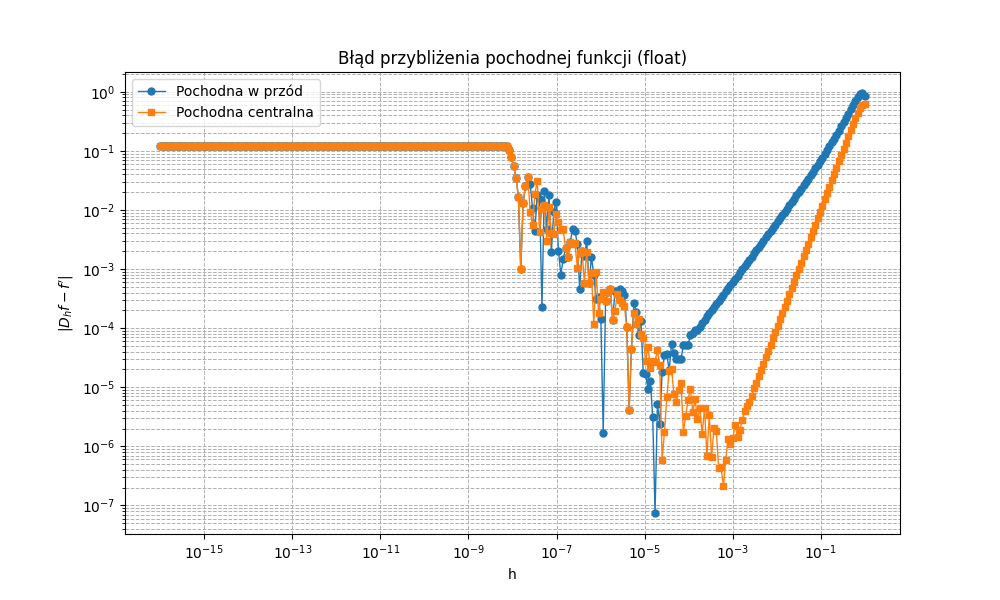
\includegraphics[width=1\textwidth]{wykres_blad_float.png}
    \caption{Błąd przybliżenia pochodnej dla zmiennej \texttt{float}.}
    \label{fig:float_error}
\end{figure}

Na wykresie \texttt{1} widać, że dla zmiennej typu \texttt{float}, metoda różnic centralnych daje mniejsze błędy niż metoda różnic w przód, szczególnie dla większych kroków \( h \). Jednakże przy bardzo małych wartościach \( h \), błąd numeryczny zaczyna rosnąć z powodu ograniczeń precyzji obliczeń.

\begin{figure}[H]
    \centering
    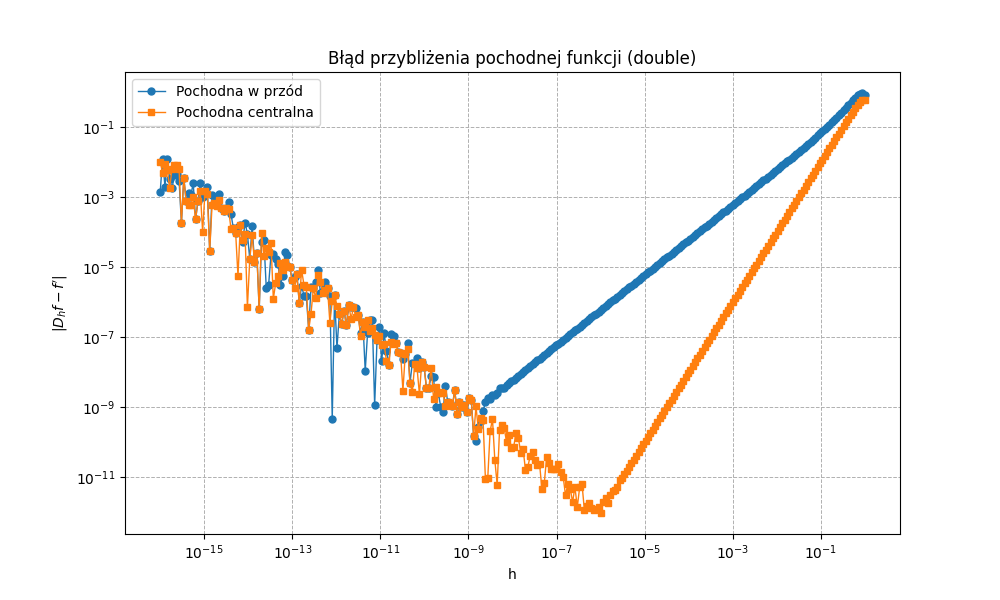
\includegraphics[width=1\textwidth]{wykres_blad_double.png}
    \caption{Błąd przybliżenia pochodnej dla zmiennej \texttt{double}.}
    \label{fig:double_error}
\end{figure}

Na wykresie \texttt{2} dla zmiennej typu \texttt{double}, błędy są mniejsze niż dla typu \texttt{float}, co wynika z wyższej precyzji obliczeń. W obu przypadkach metoda różnic centralnych oferuje lepsze przybliżenie, ale również tutaj dla bardzo małych wartości \( h \) błąd numeryczny zaczyna rosnąć.

\section{Wnioski}
Na podstawie przeprowadzonych obliczeń można stwierdzić, że:
\begin{itemize}
    \item Metoda różnic centralnych jest dokładniejsza niż metoda różnic w przód (zwłaszcza dla większych kroków \texttt{h}).
    \item Wraz ze zmniejszaniem kroku \( h \) błąd początkowo maleje. Jednak po przekroczeniu pewnej granicy rośnie z powodu ograniczeń precyzji obliczeń, szczególnie dla zmiennych typu \texttt{float}.
    \item Zmienna typu \texttt{double} oferuje większą dokładność numeryczną, co pozwala na uzyskanie lepszych wyników przy mniejszych krokach \( h \).
\end{itemize}

\end{document}

